\chapter{System Architecture and Design}

\section{System Overview}
The Flutter client communicates with organization-scoped Django API routes.
Django coordinates authentication, domain records, metric reads and writes,
and background tasks. PostgreSQL stores the operational control-plane data;
VictoriaMetrics stores time-series data; Redis supports Celery; and the
FastAPI service provides ML endpoints. Docker Compose defines these
components for local execution (\cite{compose};
\sourcepath{backend/infra_monitor/urls.py};
\sourcepath{backend/infra_monitor/organization_urls.py}).

\begin{figure}[H]
\centering
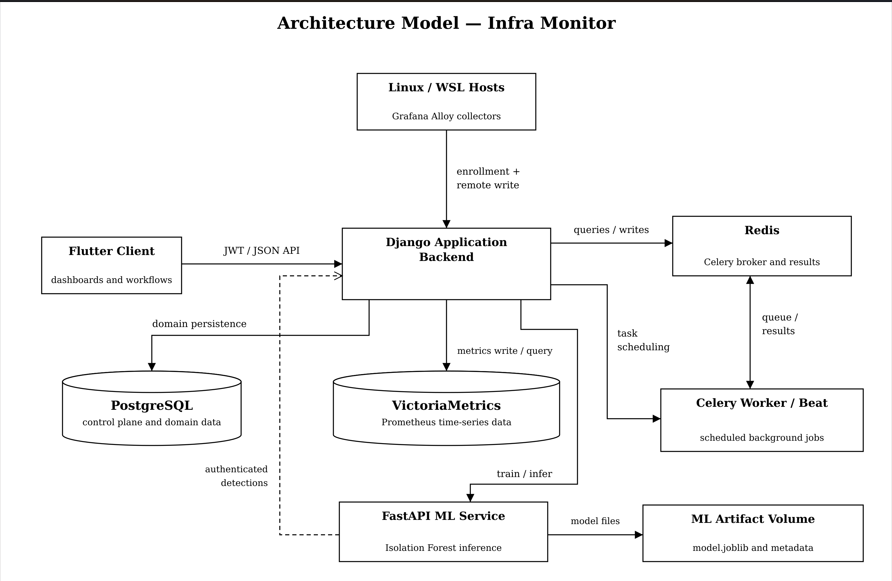
\includegraphics[width=0.88\textwidth]{assets/architecture.png}
\caption{Supplied Infra Monitor architecture diagram. The current FastAPI
service also exposes Request Shield classification, and the Gemini assistant
is implemented through Django; these paths are not drawn in this source
figure.}\label{fig:architecture}
\end{figure}

The figure is retained as a useful high-level view, but it is not a complete
deployment diagram. The model service's current routes are defined in
\sourcepath{model/app/main.py}; the conversational assistant's provider call
is in \sourcepath{backend/ai/services.py}. This distinction avoids implying
that every AI feature is hosted by the same model endpoint.

\section{Technology Stack}
\begin{table}[H]
\centering
\small
\caption{Principal technologies evidenced in the repository}\label{tab:stack}
\begin{tabularx}{\textwidth}{p{0.22\textwidth} p{0.23\textwidth} X}
\toprule
\textbf{Area} & \textbf{Technology} & \textbf{Repository evidence / role}\\
\midrule
Client & Flutter / Dart & Cross-platform interface; dependencies are declared in \sourcepath{frontend/pubspec.yaml}.\\
API and application & Django, Django REST Framework, Channels & Organization, monitoring, and workflow routes; dependency names are listed in \sourcepath{backend/requirements.txt}.\\
Operational store & PostgreSQL & Relational application data, configured as a Compose service.\\
Time-series store & VictoriaMetrics cluster & Stores/query source for Prometheus-compatible telemetry in \sourcepath{docker-compose.yml}.\\
Background work & Celery and Redis & Worker, beat scheduler, broker, and results services in \sourcepath{docker-compose.yml}.\\
ML API & FastAPI, scikit-learn & Inference/training and request classification in \sourcepath{model/app/main.py} and \sourcepath{model/requirements.txt}.\\
Host collection & Grafana Alloy & Installed on monitored Linux hosts; remote-write flow is documented in \sourcepath{docs/monitoring-end-to-end.md}.\\
\bottomrule
\end{tabularx}
\end{table}
Exact versions are stated only where pinned by manifests or image tags; the
Python requirements intentionally do not pin every package version.

\section{System Design Diagrams}
\subsection{Entity--Relationship Model}
The following black-and-white conceptual ER view uses entity boxes and
relationship diamonds. It focuses on the main organization, membership, and
monitoring records rather than drawing every supporting table. Membership is
an entity because it stores role and approval data. The relationships and
keys shown are based on Django models in
\sourcepath{backend/accounts/models/organization_membership.py},
\sourcepath{backend/servers/models/servers.py},
\sourcepath{backend/servers/models/service.py}, and
\sourcepath{backend/ml_model/models/anomaly_detection.py}.

\begin{figure}[H]
\centering
\begin{tikzpicture}[
  entity/.style={draw,rectangle,minimum width=2.8cm,minimum height=0.78cm,
                 align=center,font=\scriptsize,fill=white},
  relation/.style={draw,diamond,aspect=2,minimum width=1.25cm,
                   minimum height=0.65cm,align=center,font=\scriptsize,fill=white},
  edge/.style={draw,thick},
  card/.style={font=\scriptsize,fill=white,inner sep=1pt}
]
\node[entity] (user) at (-5,3) {USER\\id (PK), email (unique)};
\node[entity] (org) at (0,3) {ORGANIZATION\\id (PK)};
\node[entity] (server) at (5,3) {SERVER\\server\_id (PK)};
\node[entity] (membership) at (-3,0) {MEMBERSHIP\\id (PK), role, approved};
\node[entity] (service) at (5,0) {SERVICE\\service\_id (PK)};
\node[entity] (detection) at (5,-3) {ANOMALY DETECTION\\detection\_id (PK)};
\node[relation] (userMembership) at (-5,1.5) {has};
\node[relation] (orgMembership) at (-1.5,1.5) {includes};
\node[relation] (registers) at (2.5,3) {registers};
\node[relation] (hosts) at (5,1.5) {hosts};
\node[relation] (detects) at (5,-1.5) {records};
\draw[edge] (user) -- node[card,left] {1} (userMembership);
\draw[edge] (userMembership) -- node[card,left] {N} (membership);
\draw[edge] (org) -- node[card,above left] {1} (orgMembership);
\draw[edge] (orgMembership) -- node[card,below right] {N} (membership);
\draw[edge] (org) -- node[card,above] {1} (registers);
\draw[edge] (registers) -- node[card,above] {N} (server);
\draw[edge] (server) -- node[card,right] {1} (hosts);
\draw[edge] (hosts) -- node[card,right] {N} (service);
\draw[edge] (service) -- node[card,right] {1} (detects);
\draw[edge] (detects) -- node[card,right] {N} (detection);
\end{tikzpicture}
\caption{Core Infra Monitor ER model, redrawn in academic notation from backend models}\label{fig:er}
\end{figure}

\subsection{Use Cases}
The following concise use-case view was generated for this report from the
organization, server, incident, and assistant routes. It summarizes role
interactions and is not a replacement for the complete route documentation
(\sourcepath{backend/infra_monitor/organization_urls.py};
\sourcepath{backend/incident/urls.py};
\sourcepath{backend/ai/urls.py}).
\begin{figure}[H]
\centering
\begin{tikzpicture}[
  usecase/.style={draw,ellipse,minimum width=4.4cm,minimum height=0.62cm,
                  align=center,font=\small},
  actorline/.style={draw,thick},
  connect/.style={draw}
]
\draw[thick] (-3.5,-2.65) rectangle (3.5,2.65);
\node[anchor=north west,font=\small\bfseries] at (-3.35,2.55) {Infra Monitor};
\node[usecase] (login) at (0,1.85) {Authenticate};
\node[usecase] (organization) at (0,0.95) {Manage organization and members};
\node[usecase] (enroll) at (0,0.05) {Enroll monitored server};
\node[usecase] (metrics) at (0,-0.85) {View telemetry and health};
\node[usecase] (incidents) at (0,-1.75) {Review and update incidents};
\node[usecase] (assistant) at (0,-2.35) {Ask for anomaly explanation};
\draw (login.west) -- ++(-0.8,0) |- (organization.west);
\draw (login.west) -- ++(-0.45,0) |- (enroll.west);
\draw (login.east) -- ++(0.65,0) |- (metrics.east);
\draw (login.east) -- ++(0.8,0) |- (incidents.east);
\draw (login.east) -- ++(1.0,0) |- (assistant.east);
\draw[actorline] (-5.2,0.95) circle (0.18);
\draw[actorline] (-5.2,0.77) -- (-5.2,0.0);
\draw[actorline] (-5.2,0.55) -- (-5.55,0.25);
\draw[actorline] (-5.2,0.55) -- (-4.85,0.25);
\draw[actorline] (-5.2,0.0) -- (-5.5,-0.38);
\draw[actorline] (-5.2,0.0) -- (-4.9,-0.38);
\node[align=center,font=\small] at (-5.2,-0.7) {Owner / Admin};
\draw[actorline] (5.2,0.95) circle (0.18);
\draw[actorline] (5.2,0.77) -- (5.2,0.0);
\draw[actorline] (5.2,0.55) -- (4.85,0.25);
\draw[actorline] (5.2,0.55) -- (5.55,0.25);
\draw[actorline] (5.2,0.0) -- (4.9,-0.38);
\draw[actorline] (5.2,0.0) -- (5.5,-0.38);
\node[align=center,font=\small] at (5.2,-0.7) {Engineer};
\draw[connect] (-4.8,0.6) -- (login.west);
\draw[connect] (-4.8,0.6) -- (organization.west);
\draw[connect] (-4.8,0.6) -- (enroll.west);
\draw[connect] (4.8,0.6) -- (login.east);
\draw[connect] (4.8,0.6) -- (metrics.east);
\draw[connect] (4.8,0.6) -- (incidents.east);
\draw[connect] (4.8,0.6) -- (assistant.east);
\end{tikzpicture}
\caption{Report-generated use-case summary from current application routes}\label{fig:usecases}
\end{figure}

\section{Database Schema}
The application separates identity and organization membership from monitoring
objects. A user can participate in organizations through a membership with
role and approval state; an organization owns servers; a server contains
services; and anomaly records reference the organization, server, and
optionally a service. Alerts and incidents are separate operational records
with organization and server/service references
(\sourcepath{backend/accounts/models/organization_membership.py};
\sourcepath{backend/alert/models/alert.py};
\sourcepath{backend/incident/models/incident.py}).

\begin{table}[H]
\centering
\small
\caption{Selected domain records and key relationships}\label{tab:schema}
\begin{tabularx}{\textwidth}{p{0.22\textwidth} p{0.28\textwidth} X}
\toprule
\textbf{Record} & \textbf{Key fields} & \textbf{Relationship / constraint}\\
\midrule
Organization & UUID primary key, name & Parent scope for servers, memberships, alerts, incidents, and detections.\\
OrganizationMembership & UUID key, user FK, organization FK, role, approved & Unique per user and organization; approved privileged roles are constrained.\\
Server & UUID key, organization FK, host name, environment, status & Host name is unique within an organization.\\
Service & UUID key, server FK, service name, status & Service name is unique within a server.\\
AnomalyDetection & UUID key, organization/server/service FKs, scores, feature values, window & Model-version and time-window uniqueness per service.\\
Alert / Incident & UUID keys, organization and optional server/service references & Lifecycle state, severity, and assignment fields support operations.\\
\bottomrule
\end{tabularx}
\end{table}

\section{User Interface Design}
The supplied Flutter screenshots show a dashboard overview, server inventory,
metric detail, and incident queue. They are illustrative interface captures,
not evidence of a formal user-acceptance test or measured production state.
The screen composition is implemented in the Flutter client under
\sourcepath{frontend/lib/}.

\begin{figure}[H]
\centering
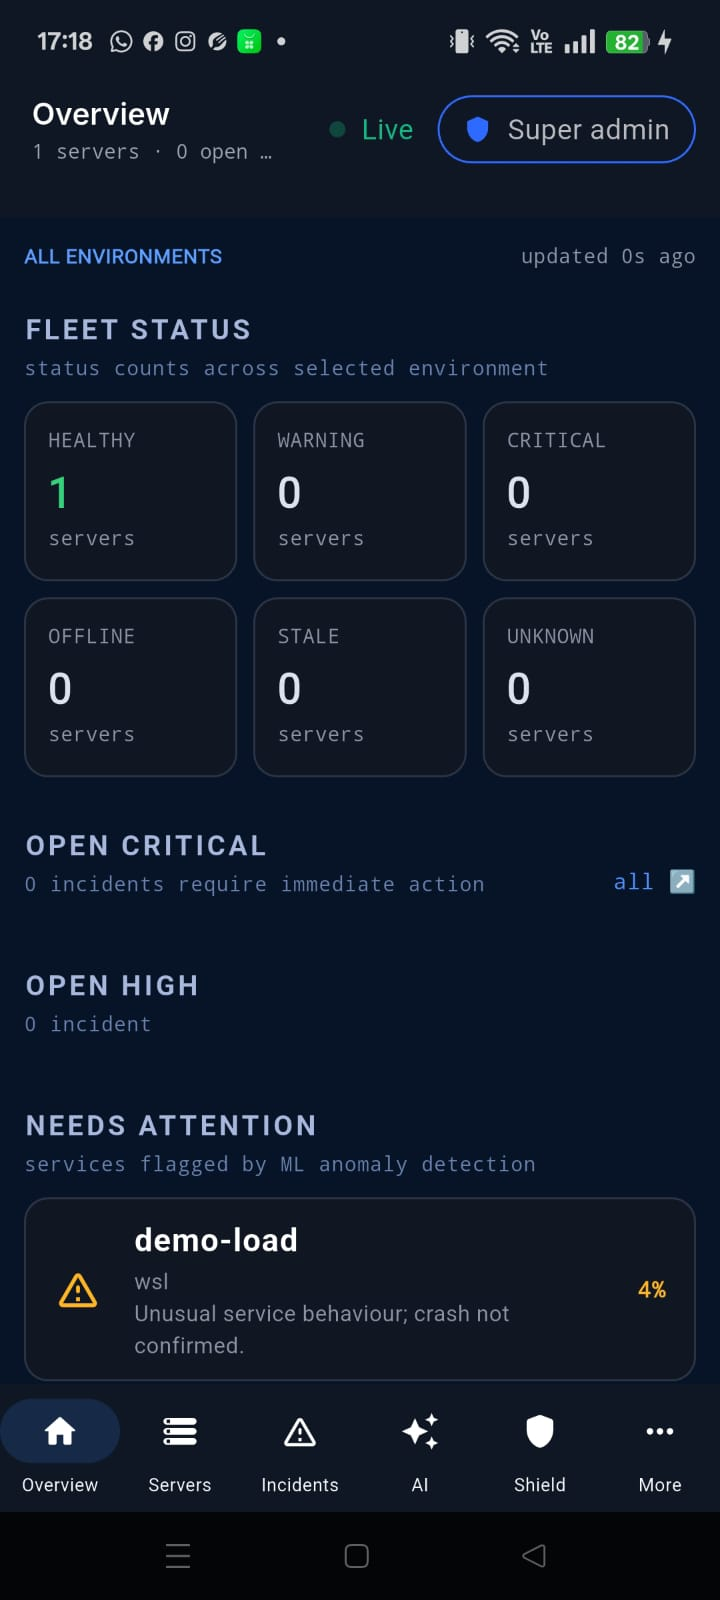
\includegraphics[width=0.29\textwidth,height=0.36\textheight,keepaspectratio]{assets/ui_overview.jpeg}
\hfill
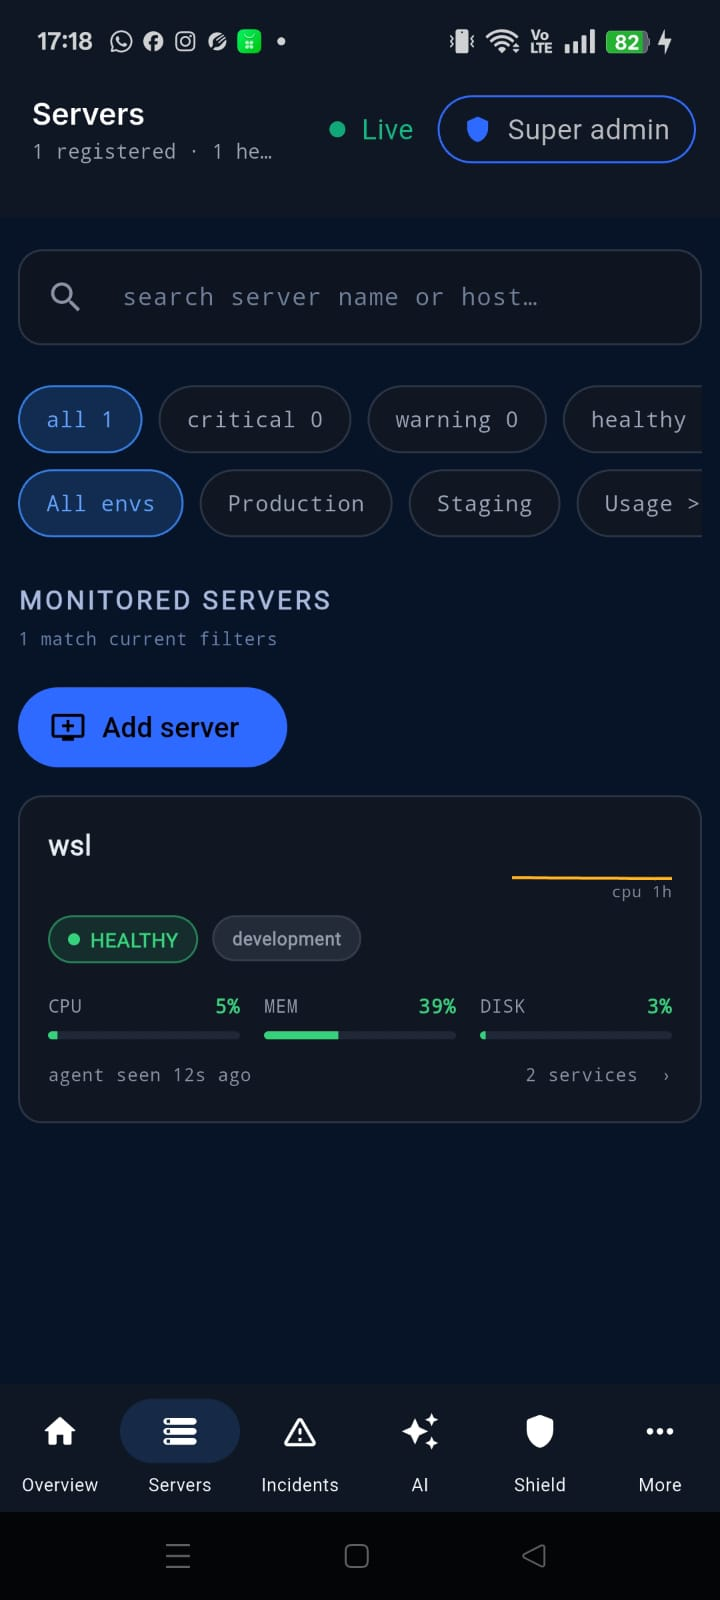
\includegraphics[width=0.29\textwidth,height=0.36\textheight,keepaspectratio]{assets/ui_servers.jpeg}
\caption{Dashboard overview (left) and monitored server list (right)}\label{fig:ui-overview}
\end{figure}
\begin{figure}[H]
\centering
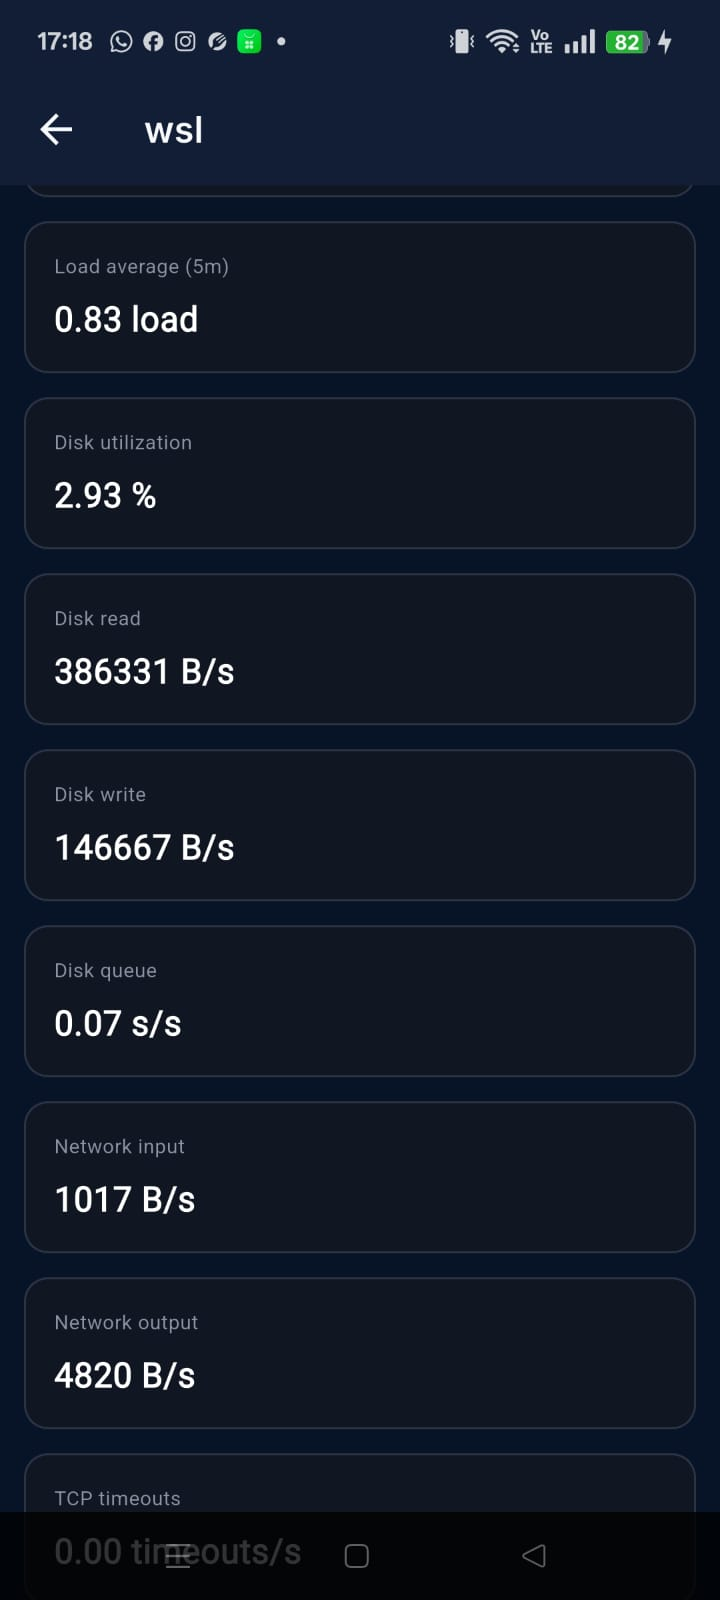
\includegraphics[width=0.29\textwidth,height=0.36\textheight,keepaspectratio]{assets/ui_metrics.jpeg}
\hfill
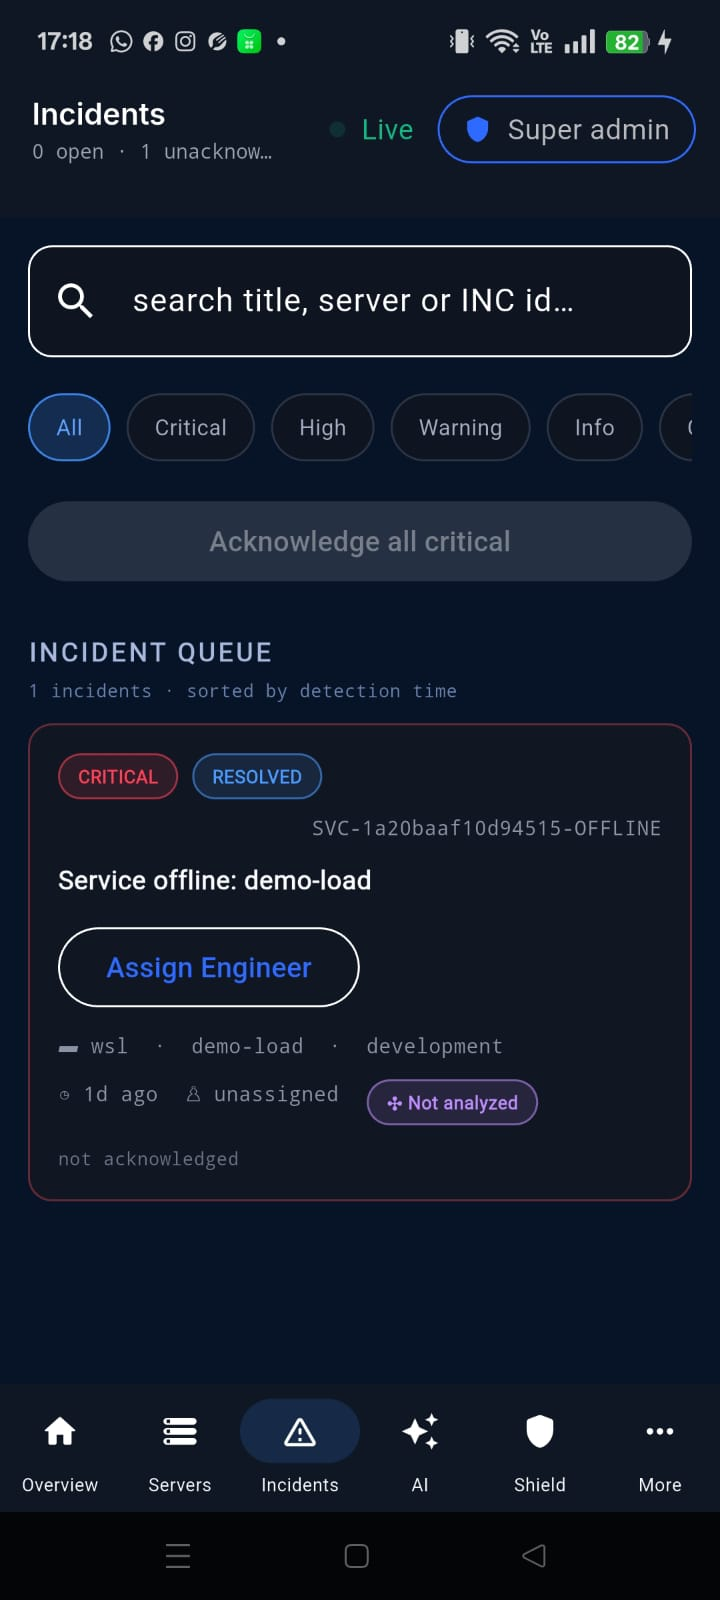
\includegraphics[width=0.29\textwidth,height=0.36\textheight,keepaspectratio]{assets/ui_incidents.jpeg}
\caption{Service metric detail (left) and incident queue (right)}\label{fig:ui-operations}
\end{figure}
